Below is an outline for this section.

\begin{enumerate}

\item Brief summary of results
\item Interpretation of results
\begin{enumerate}
	\item It is possible that the programs shared more features as they evolved. See Figures~\ref{fig:agg-admin} and~\ref{fig:agg-ped} for a visualization of the similarities and differences between the programs. Using results from the structured interviews, we compute the number of administrative and pedagogical components that each program shares with the Reggio Approach by school type, city, and year. We examine 14 administrative components and 12 pedagogical components. Over time, many of the programs other than the state programs, adopt more features present in the Reggio Approach. This is especially true of the Parma municipal program.
	\item Expand discussion of survey highlighting specific questions that presented interesting results
\end{enumerate}

\item Issues with these results
\begin{enumerate}
	\item Selection issues
	\begin{enumerate}
		\item With more background variables for the adult cohorts, matching might be more successful
		\item With more accurate information on the distance to the nearest school, an instrumental variable approach might work
		\item Complete information on tuition costs would help understand the selection
		\item Discuss differences in eligibility requirements between cities and schools and how that might have contributed to differential selection
	\end{enumerate}
	\item Data issues
\end{enumerate}

\end{enumerate}

\begin{figure}
\begin{center}
\caption{Number of Administrative Characteristics in Common with the Reggio Approach}
\label{fig:agg-admin}
	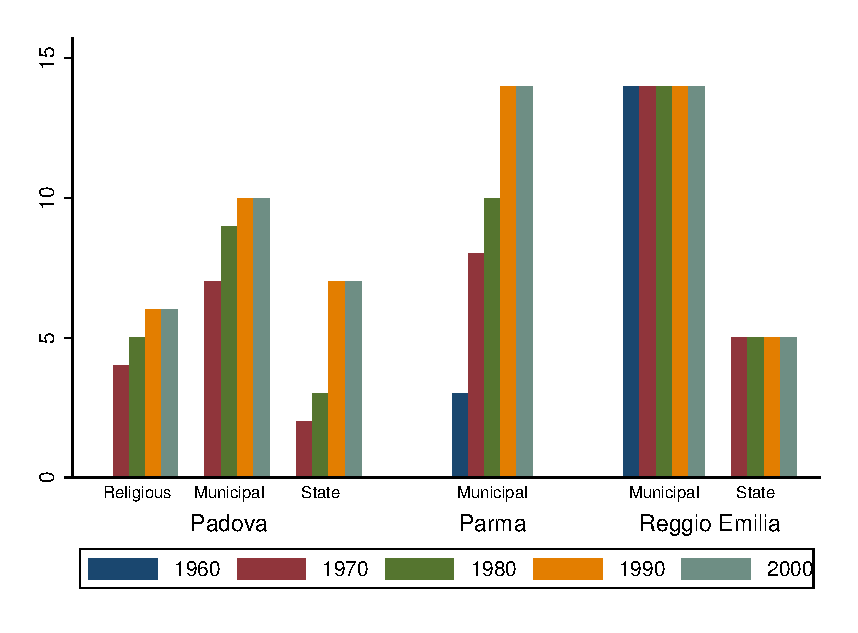
\includegraphics[width=0.8\textwidth]{../../output/aggregateAdministrative.eps}
\end{center}
\raggedright \footnotesize Note: This graph shows the number of administrative components that each program has in common with the Reggio Approach. We consider 14 administrative components. 
\end{figure}


\begin{figure}
\begin{center}
\caption{Number of Pedagogical Characteristics in Common with the Reggio Approach}
\label{fig:agg-ped}
	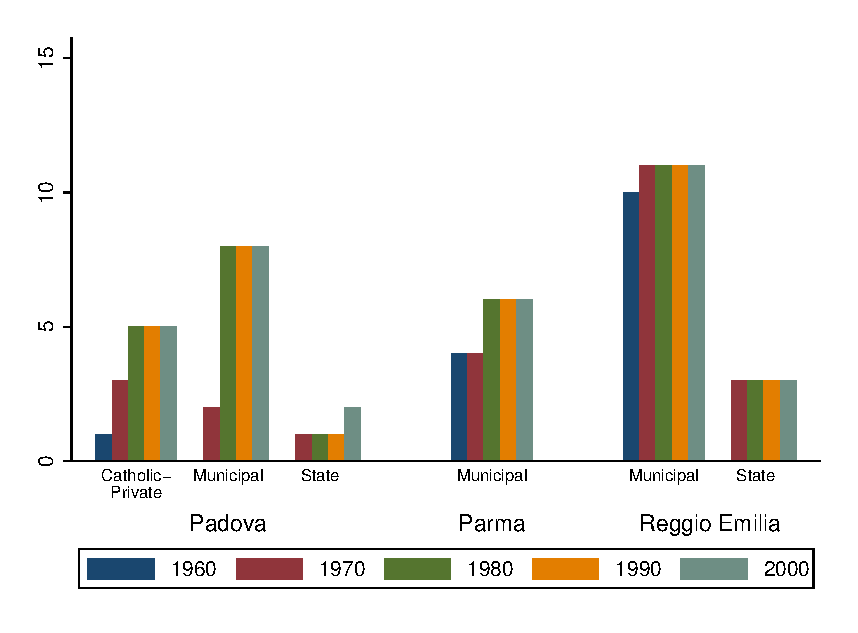
\includegraphics[width=0.8\textwidth]{../../output/aggregatePedagogical.eps}
\end{center}
	\raggedright \footnotesize Note: This graph shows the number of pedagogical components that each program has in common with the Reggio Approach. We consider 12 pedagogical components. 
	\end{figure}